\chapter{Strumenti}
Per analizzare le varie architetture presentate dobbiamo prima fare un discorso sugli strumenti utilizzati per costruire una applicazione web e che useremo per gli esempi di codice dei capitoli successivi.

\section{ECMAScript 2015}
Anche conosciuto come \textit{ECMAScript6}, è una standardizzazione del linguaggio Javascript creata da Ecma International. Questa versione in particolare mette a disposizione features molto utili per scrivere codice funzionale. Possiamo classificare ECMAScript come un linguaggio a sé e differente da Javascript, che in principio doveva essere utilizzato solamente come linguaggio di scripting lato web, ma che ora viene utilizzato come vero e proprio linguaggio di programmazione su ambienti e scale differenti \cite{ECMAScriptDocumentation}.

In ambito web non tutte le features di ES6 sono disponibili, per questo si utilizzano strumenti come \textit{Babel} o \textit{Webpack} che hanno la funzione di \textit{transpiler}, ossia di compilare codice sorgente da ECMAScript6 a ECMAScript5 che è supportato dalla stragrande maggioranza dei browser.

Le funzionalità introdotte da ECMAScript6 sono molte, tuttavia qui parleremo solo di quelle che risulteranno propedeutiche per capire i pezzi di codice nei capitoli successivi.

\subsection{Let e Const}
Una delle features introdotte, che probabilmente è anche una delle più incisive, riguarda l'assegnazione delle variabili. In ES5 la dichiarazione avveniva tramite la keyword \textit{var} ed il loro scope era relativo alla funzione direttamente loro superiore.
 
\begin{listing}[ht]
\inputminted{Javascript}{sources/exampleVarES5.js}
\caption{Esempio della dichiarazione di una variabile con \textit{var}.}
\end{listing}

\noindent
In ES6 a questa si aggiungono anche \text{let} e \textit{const} il cui scope è relativo al blocco in cui sono posizionate (e non alla funzione, come in \textit{var}). La prima non ha nulla di particolare oltre ciò che abbiamo già detto, la seconda invece dichiara variabili costanti, ossia il cui valore non può mutare.

\begin{listing}[ht]
\inputminted{Javascript}{sources/exampleLetConstES6.js}
\caption{Esempio della dichiarazione di variabili con \textit{let} e \textit{const}.}
\end{listing}

\noindent
La keyword \textit{const} verrà molto utilizzata nei successivi codici in quanto costituisce un concetto fondamentale dei linguaggi funzionali: l'immutabilità\footnotemark.

\subsection{Arrow Function}
In ES5 bisogna prestare attenzione all'utilizzo di \textit{this} quando stiamo utilizzando l'espressione \textit{function} in quanto potremmo non ottenere cosa ci aspettiamo.

\begin{listing}[ht]
\inputminted{Javascript}{sources/exampleShadowThisES5.js}
\caption{Esempio di comportamento inaspettato di \textit{this}.}
\end{listing}

\noindent
Questo capita perché il costrutto \textit{function} ha uno scope proprio, e quindi la variabile \textit{this} viene sovrascritta. Per evitare ciò ES6 mette a disposizione le \textit{Arrow Function}, ossia funzioni anonime che non sovrascrivono il \textit{this} ereditato.

\begin{listing}[ht]
\inputminted{Javascript}{sources/exampleArrowFunctionES6.js}
\caption{Esempio di \textit{Arrow Function}.}
\end{listing} 

\footnotetext{Il concetto di immutabilità è un pilastro fondamentale della programmazione funzionale, e rappresenta un oggetto il cui stato non può essere modificato in alcun modo. Avere un elemento immutabile significa che l'unico modo per modificarlo è quello di crearne uno nuovo con le modifiche volute e modificare la referenza a quest'ultimo.}

\subsection{Parametri di default ed a oggetti}
ES6 ci permette di utilizzare valori predefiniti per i parametri delle funzioni che creiamo. Questi valori di default vengono assegnati quando i normali parametri sono \textit{undefined}. 

\begin{listing}[ht]
\inputminted{Javascript}{sources/exampleDefaultParametersES6.js}
\caption{Esempio di utilizzo dei parametri di default.}
\end{listing}

\noindent
Un altro miglioramento apportato da ES6 riguarda gli oggetti passati come parametri. E' ora possibile destrutturare un oggetto direttamente dai parametri durante la definizione di una funzione.

\begin{listing}[ht]
\inputminted{Javascript}{sources/exampleObjectParameterES6.js}
\caption{Esempio di destrutturazione di un oggetto passato come parametro.}
\end{listing}

\subsection{Classi}
In Javascript non esistono classi, esistono invece oggetti con proprietà particolari che ci permettono di simulare ereditarietà e riusabilità. ES5 non possiede una vera e propria parola chiave per definire una classe, e quindi per creare un oggetto che si comporti come tale partiamo dal costruttore per poi aggiungere i metodi voluti \cite{RylanOnPrototypeInheritance}.

\begin{listing}[ht]
\inputminted{Javascript}{sources/examplePrototypeInheritanceES5.js}
\caption{Esempio di una classe in ES5.}
\end{listing}

\noindent
ES6 ci mette a disposizione una sintassi molto più comprensibile e versatile per la gestione delle classi, che però fa sempre capo al vecchio concetto di ES5 (non esiste una vera e propria classe quindi, neanche in ES6). 

\begin{listing}[ht]
\inputminted{Javascript}{sources/exampleClassES6.js}
\caption{Esempio di una classe in ES6.}
\end{listing}

\subsection{Struttura statica dei moduli}
La struttura dei moduli di ES5, usando ad esempio la sintassi di \textit{CommonJS}\footnotemark, è dinamica ciò significa che l'importazione e l'esportazione avviene in maniera dinamica ed in run-time. Questo comporta che per analizzare le dipendenze di un progetto ed eliminare eventuale codice non utilizzato, è obbligatoriamente necessario eseguire il codice e monitorarne il comportamento.

\begin{listing}[ht]
\inputminted{Javascript}{sources/exampleDynamicImportES5.js}
\caption{Esempio di importazione dinamica di un modulo in ES5.} 
\end{listing}

\noindent
ES6 mette a disposizione un sistema di gestione dei moduli statico. Questo comporta la possibilità di analizzare le dipendenze di un codice in compile-time e la possibilità quindi di eliminare tutto ciò che non viene effettivamente utilizzato.
Tuttavia non abbiamo più la libertà dei moduli non nativi e c'è la necessità di attenersi a delle regole come ad esempio l'obbligo di effettuare le importazione e le esportazioni al livello più alto del codice e non all'interno di qualche blocco, e sopratutto non devono essere presenti elementi dinamici (come ad esempio variabili).

\begin{listing}[ht]
\inputminted{Javascript}{sources/exampleImportExportES6.js}
\caption{Esempio di importazione statica di un modulo in ES6.}  
\end{listing}

\footnotetext{CommonJS definisce un formato per l'utilizzo dei moduli su Javascript.}

\section{Webpack}
Abbiamo parlato nella sezione precedente di Webpack e di come è in grado di trasformare ECMAScript 6 nella sua precedente versione supportata da quasi tutti i browser attuali. Tuttavia questa è solo una piccola caratteristica rispetto a quello che è veramente.
Nel sito ufficiale Webpack è descritto come \blockquote{A module bundler for modern JavaScript applications.} in pratica si occupa di ricercare tutte le dipendenze dell'applicazione e raggrupparle in un unico file. 
Per capire a pieno questo concetto è bene analizzare la struttura di una applicazione Javascript moderna che normalmente consideriamo divisa in due parti ben distinte: il codice sorgente di base e i moduli (sia propri che di terzi) che implementano le varie funzioni. Un modulo è una unità dell'applicazione che contiene tutto il necessario per eseguire un aspetto o una particolare funzionalità di essa. Un modulo può includere dentro di se una o più librerie, ossia delle collezioni di funzioni e metodi per risolvere dei particolari problemi. Quello che fa Webpack è analizzare il file Javascript relativo alla nostra applicazione, chiamato "Entry point", e creare un pacchetto con tutti i moduli e le librerie affinché il servizio possa funzionare in maniera corretta. 

Con Webpack diventa estremamente facile suddividere l'applicazione in files di dipendenze multipli che possono includere da codici sorgenti come moduli Javascript o CSS, fino ad immagini e font.
E' anche possibile utilizzare \textit{Loader}, ossia dei middleware, che prendono in input delle dipendenze specifiche e le trasformano a seconda di ciò che abbiamo bisogno (Il transpiler da ES6 ad ES5 è esattamente questo prendendo in input ogni file Javascript).

\begin{figure}[h]
\centering
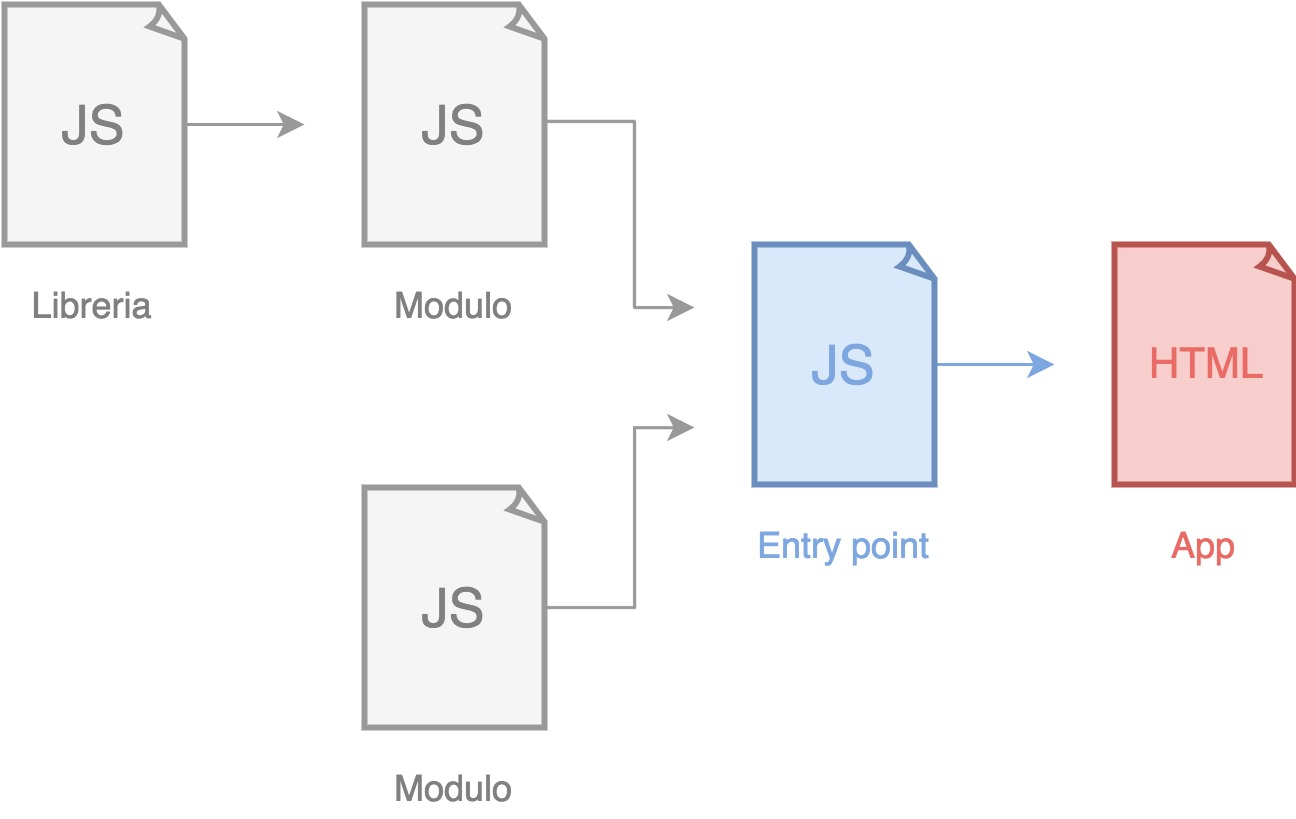
\includegraphics[width=10cm]{./images/webpackWorkflow}
\caption{Rappresentazione del sistema di impacchettamento di Webpack.}
\end{figure}

\subsection{Hot Module Replacement}
Un aspetto molto interessante di Webpack riguarda l'\textit{Hot Module Replacement} (HMR) che si occupa di aggiungere o rimuovere i pacchetti di dipendenze generati nel run-time dell'applicazione senza un aggiornamento completo della pagina. Questo è molto utile in fase di development in quanto consente di mantenere lo stato di una applicazione anche dopo aver effettuato modifiche al sorgente ed avere le nuove caratteristiche disponibili in maniera molto più veloce del normale aggiornando solo ciò che è necessario. 

\subsection{Tree Shaking}
La tecnica del \textit{Tree Shaking} permette di eliminare il codice inutilizzato all'interno della codebase. Quello che fa Webpack è andare ad analizzare a la struttura di \textit{Import} ed \textit{Export} del sorgente che, come abbiamo detto precedentemente nella sezione riguardante ES6, è statica ossia è possibile analizzarla a \textit{compile-time} senza la necessità di eseguire il codice. Una volta trovati gli elementi che non vengono utilizzati essi vengono classificati come “codice morto" e vengono marcati attraverso adeguati commenti. Webpack non si occupa di eliminare questi elementi ma affida il compito ad un eventuale \textit{Minifier} (come ad esempio \textit{UglifyJS}) che si occupa di ottimizzare il codice Javascript.

\section{React}
React è una libreria scritta da Facebook per la creazione di interfacce utente interattive in maniera funzionale ed altamente scalabile. Si basa sul concetto di "componente" come elemento base fondamentale, ossia un pezzo di interfaccia che ha uno stato proprio ed è riutilizzabile all'interno del servizio. Il concetto funzionale di composizione si adatta benissimo a React: un componente complesso dovrebbe essere formato da componenti più piccoli e agnostici che possono quindi essere riutilizzati in altri componenti complessi.

Viene utilizzato in produzione sia da Facebook che da Instagram e fa uso di diverse tecnologie all'avanguardia come il \textit{Virtual DOM} ed il \textit{Server-side Rendering} \cite{WheelerOnReact}.

\subsection{Virtual DOM}
Il  \textit{Document Object Model} (DOM) è una API che definisce la struttura di un documento HTML e come essa viene acceduta e manipolata. E' una rappresentazione ad oggetti di una pagina web la quale può essere modificata con un linguaggio di scripting come Javascript.
Per fare un esempio pratico, lo standard DOM stabilisce che l'interfaccia \textit{Document} rappresenti l'intera pagina HTML e che concettualmente sia il nodo root. L'interfaccia \textit{Node} rappresenta invece l'elemento base ossia il singolo nodo all'interno di un documento e l'implementazione di questa richiede la creazione dei metodi per la gestione del nodo stesso e dei propri figli \cite{HWRWhatIsDOM}.

Quando parliamo di Virtual DOM parliamo di un'astrazione sopra l'astrazione del DOM. Modificare quest'ultimo non è particolarmente dispendioso (si tratta solamente di modificare un oggetto Javascript) è tuttavia il processo di lettura e di “ridisegno" della pagina da parte del browser il vero problema. Questa tecnologia riesce a risolvere il suddetto problema mantenendo in memoria una rappresentazione del DOM reale che utilizza il design pattern \textit{Observer}\footnotemark per capire quale particolare nodo è stato modificato generando successivamente un nuovo albero derivato dal precedente ma con il nuovo stato. A questo punto effettua complessi algoritmi di differenza per trovare il numero minimo di passaggi per aggiornare il DOM reale per poter infine effettuare la riconciliazione \cite{MishraOnVirtualDOM}.

Il concetto che permette al Virtual DOM di garantire prestazioni maggiori sul DOM reale consiste nell'aggiornamento aggregato. Tutti i cambiamenti effettuati da un evento (che sono i passaggi trovati dall'algoritmo di differenza) vengono aggregati ed il DOM viene ridisegnato solamente una volta.

React implementa il Virtual DOM attraverso \textit{JSX}, una estensione di ECMAScript simile ad XML che permette di scrivere elementi di markup con una sintassi simile all'HTML all'interno dei componenti dell'interfaccia. Portare l'HTML all'interno del codice sorgente Javascript offre dei vantaggi non banali come ad esempio il debugging compile-time degli errori di sintassi durante la costruzione del DOM, la versatilità di avere un linguaggio di scripting per effettuare composizione ed altre azioni dinamiche e sopratutto avere una perfetta separazione tra componenti differenti.

\footnotetext{Il design pattern Observer si struttura di un oggetto chiamato “Subject" che mantiene una lista di altri oggetti dipendenti chiamati "Observers" e li notifica ogni qualvolta il suo stato viene modificato.}

\subsection{Server-side rendering}
React è una libreria \textit{isomorfica}, è in grado di essere eseguita sia lato client che lato server traendo vantaggio da NodeJS ed il fatto che il principale linguaggio di programmazione per entrambi gli ambienti sia sempre Javascript.
Il vantaggio di eseguire React anche lato server risiede nella prima visualizzazione. In una Single Page Application normale durante il primo caricamento vengono scaricati gli elementi base per la sua esecuzione e successivamente viene eseguito il codice Javascript per il rendering del suo stato iniziale. La seconda fase può essere ulteriormente pesante, basti pensare che possono essere effettuate ulteriori richieste per soddisfare il normale fabbisogno dell'applicazione.

La tecnica del Server-side rendering permette di semplificare questa prima visualizzazione interpretando i componenti React lato server e restituendo una pagina iniziale con la Single Page Application già avviata e fornita di tutti i dati di cui avrebbe normalmente bisogno.